%! Author = arqfa
%! Date = 8/8/2023

% Preamble
%\documentclass[11pt]{article}
\documentclass[final,5p,times]{elsarticle}
% Packages
%% The amssymb package provides various useful mathematical symbols
\usepackage{amssymb}
%% The amsthm package provides extended theorem environments
\usepackage{amsthm}
\usepackage{graphicx}
\usepackage{tabularx}
\usepackage{booktabs}
%% The lineno packages adds line numbers. Start line numbering with
%%\begin{linenumbers}, end it with \end{linenumbers}. Or switch it on
%% for the whole article with \linenumbers
\usepackage{lineno}
\modulolinenumbers[10]
\usepackage{enumitem}

\usepackage{multirow}

\usepackage{caption}

\journal{Computer Aid Design}


% Document
\begin{document}

\begin{frontmatter}


\title{Embracing Complexity: Mixed Reality Assessment of User Tolerance for Complex Facades in Future Construction Trends}

%% use optional labels to link authors explicitly to addresses:
%% \author[label1,label2]{}
%% \affiliation[label1]{organization={},
%%             addressline={},
%%             city={},
%%             postcode={},
%%             state={},
%%             country={}}
%%
%% \affiliation[label2]{organization={},
%%             addressline={},
%%             city={},
%%             postcode={},
%%             state={},
%%             country={}}

\author[inst1]{Fabian Jarrin}
\author[inst1]{Yasuko Koga}
\author[inst2]{Diego Thomas}

\affiliation[inst1]{organization={Graduate School of Human-Environment Studies, Department of Architecture and Urban Design, Kyushu University},%Department and Organization
            addressline={744 Motooka, Nishi Ward},
            city={Fukuoka},
            postcode={819-0382},
            state={Kyushu},
            country={Japan}}

\affiliation[inst2]{organization={Graduate School of Information Science and Electrical Engineering, Kyushu University},%Department and Organization
            addressline={744 Motooka, Nishi Ward},
            city={Fukuoka},
            postcode={819-0382},
            state={Kyushu},
            country={Japan}}

\begin{abstract}
%% Text of abstract
This research aims to evaluate the efficacy of virtual reality (VR) simulations in promoting the acceptance of data-driven optimized design solutions for Site Layout Planning (SLP). The study involves the development of a multi-objective optimization model, considering essential factors such as earthwork volume calculations, cost, and environmental impact, particularly for an educational building located on the site. The model is subsequently transformed into an interactive VR simulation, enabling participants to visually observe the real-time impact of various building placements on the site. The results indicate that the utilization of the VR simulation significantly enhances the understanding and acceptance of the recommended data-driven optimized design solutions. On average, participants experienced a notable \(48.3\%\) increase in accuracy compared to traditional methods. The technology was highly regarded by participants, receiving an average acceptance rate of 5.4 on a 7-point Likert scale. It is essential to recognize that while VR simulations show promise in expediting the adoption of data-driven optimized design solutions, they are not intended to replace existing design review methods. Instead, they serve as a means to streamline the decision-making process and provide stakeholders with a more immersive and comprehensive understanding of the design solutions.

        %This research focuses on assessing the effectiveness of virtual reality (VR) simulations in promoting the acceptance of data-driven optimized design solutions for Site Layout Planning (SLP). To achieve this, a multi-objective optimization model was developed, taking into account important factors such as earthwork volume calculations, cost, and environmental impact, particularly for an educational building situated on the site. The model was then transformed into an interactive VR simulation, allowing participants to visually observe the real-time consequences of different building placements on the site. 
        %The findings of the research indicate that the utilization of the VR simulation significantly enhanced the understanding and acceptance of the recommended data-driven optimized design solutions. On average, participants experienced a notable \(48.3\%\) increase in accuracy when compared to traditional methods. The technology itself was highly regarded by participants, receiving an average acceptance rate of 5.4, across several levels, on a 7-point Likert scale.
        %It is important to note that while VR simulations show promise in expediting the adoption of data-driven optimized design solutions, they are not meant to replace existing design review methods. Instead, they serve as a means to streamline the decision-making process and provide stakeholders with a more immersive and comprehensive understanding of the design solutions.
        


\end{abstract}


%%Graphical abstract

\begin{graphicalabstract}
    \centering
    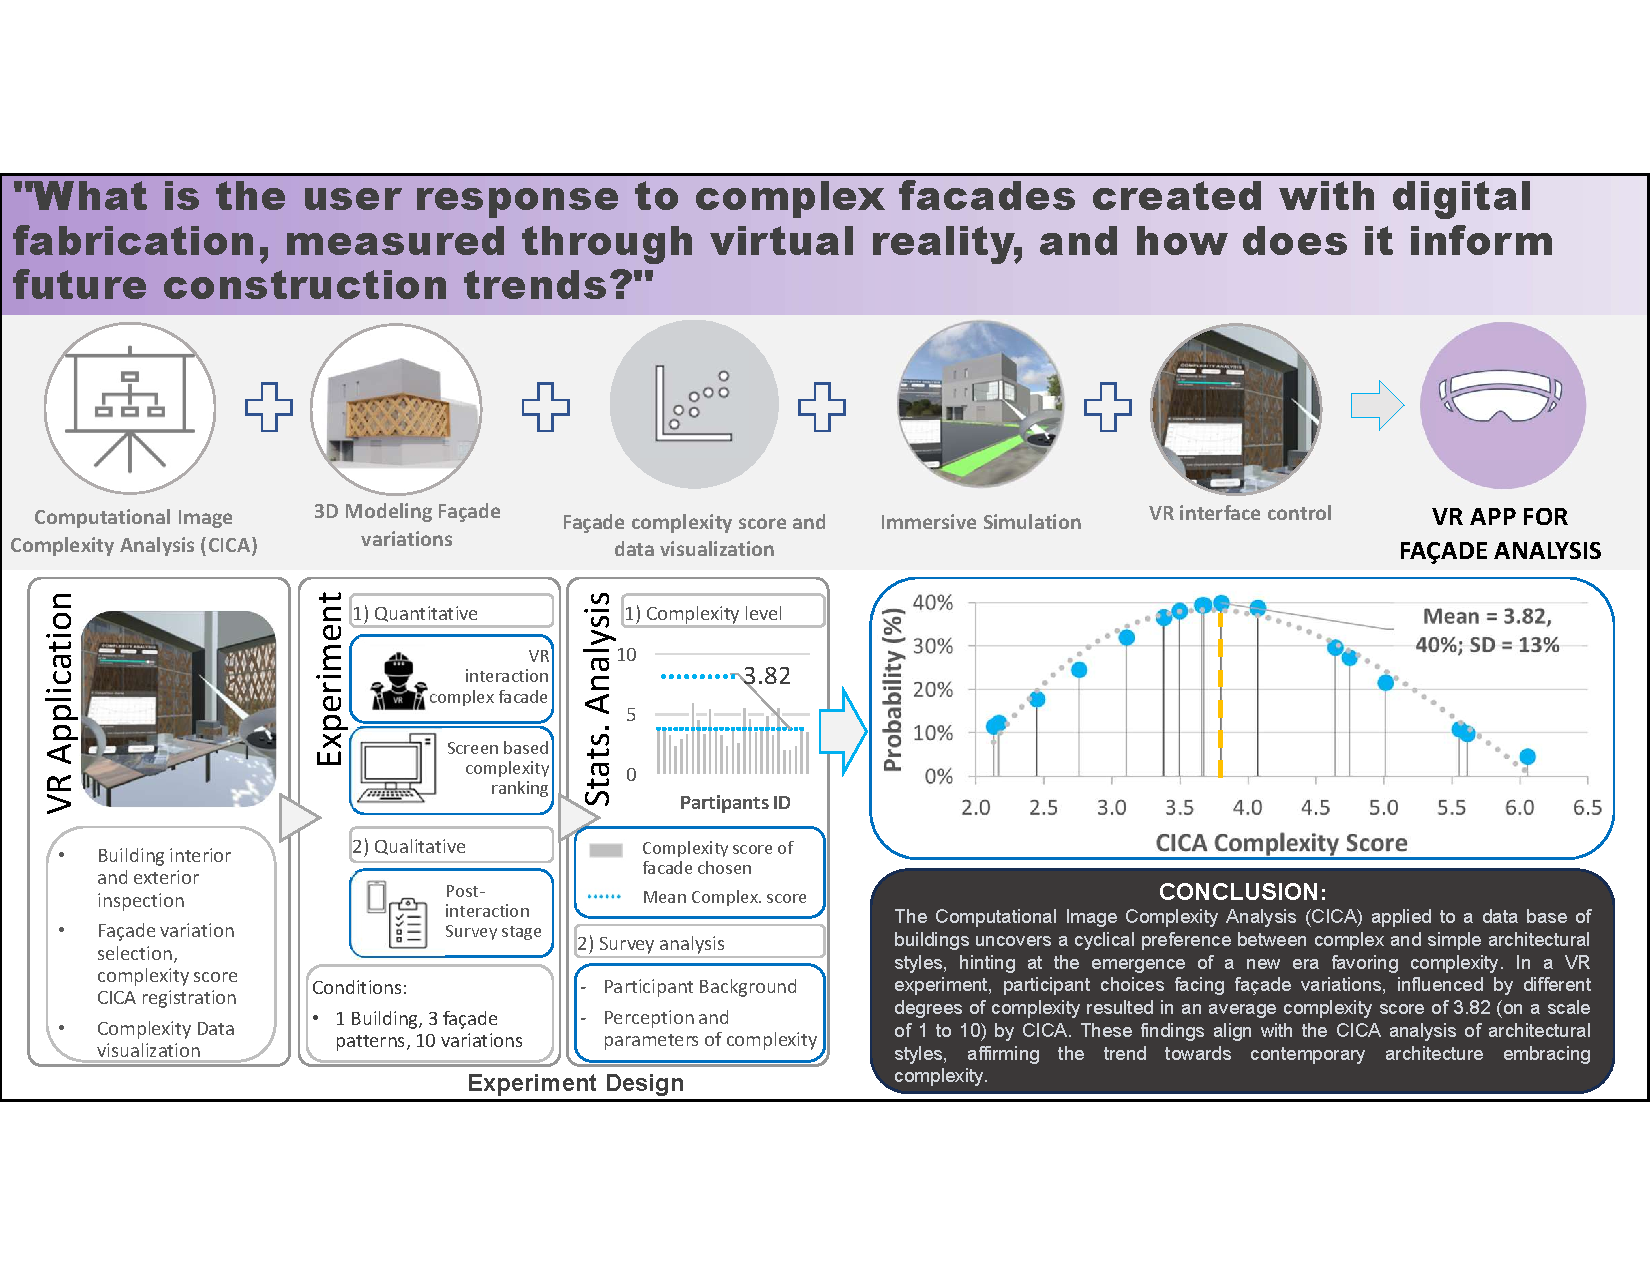
\includegraphics[width= \textwidth, trim = 0 80 0 80, clip]{Images/GraphicAbstract}
    \label{fig:graphic_abstract}
\end{graphicalabstract}

%%Research highlights
\begin{highlights}
%highlights

\item Computational Image Complexity Analysis (CICA) system using computer vision.
\item CICA system quantifies facade complexity, aiding in historical trend analysis.
\item VR experiment indicates user preference for moderate complexity in facades.
\item Future architecture favoring user-centric, complexity balanced designs trends.

\end{highlights}

\begin{keyword}
%% keywords here, in the form: keyword \sep keyword
Data-driven design\sep Site Layout Planning \sep Virtual reality \sep Optimization\sep

\end{keyword}

\end{frontmatter}
%\linenumbers
%\modulolinenumbers[10]
%
\begin{linenumbers}


\section{Introduction}
\label{sec:1Introduction}
%%State the objectives of the work and provide an adequate background, avoiding a detailed literature survey or a summary of the results.
%%Introduction

%=================================
%%Reference
%%https://www.scribbr.com/research-paper/research-paper-introduction/
%%State the objectives of the work and provide an adequate background, avoiding a detailed literature survey or a summary of the results.

%Step1. Introduce your topic.
     %This is generally accomplished with a strong opening hook.
%Step2. Describe the background.
     %For a paper describing original research, you’ll instead provide an overview of the most relevant research that has already been conducted.
%Step3. Establish your research problem.
     %In an empirical research paper, try to lead into the problem on the basis of your discussion of the literature.
%Step4. Specify your objective(s).
     %The research question is the question you want to answer in an empirical research paper. If your research involved testing hypotheses, these should be stated along with your research question.
%Step 5: Map out your paper.
     %The final part of the introduction is often dedicated to a brief overview of the rest of the paper.

%recommended limit 500 words
%=================================

Recent advancements in Building Information Modeling (BIM) and digital fabrication are transforming architectural practice.
These technologies enable architects to design intricate and complex forms, moving beyond the uniformity of barren walls and fully glazed facades that often dominate contemporary streetscapes.
By leveraging these advancements, architects can introduce complexity and detail into their designs, enhancing both the visual and functional aspects of buildings, and creating more engaging and dynamic environments that potentially redefine the relationship between form and function~\cite{Leach2016}.

However, the pursuit of complexity in architectural design must be balanced with sustainability and user satisfaction.
Designs that are overly complex without consideration of these factors can quickly become outdated and disconnected from their inhabitants, leading to issues of obsolescence and lack of relevance~\cite{Oberfrancova2021}.
Understanding how complexity can enhance both environmental sustainability and user satisfaction is therefore crucial for modern architectural practice.

Previous research has extensively explored the impact of complexity in architectural design, identifying mathematical relationships between complexity and aesthetic value ~\cite{Bies2016, Douchova2016, Redies2015}.
Despite these insights, the architectural field has yet to develop frameworks that leverage these principles for practical design applications, especially considering modern technological advancements aimed at sustainability.

This study aims to bridge the gap between theoretical understanding and practical application by developing a methodology to measure facade complexity.
The objectives are to generate data that can improve `Data-driven Building Design' (DBD) by integrating a complexity scoring function that can inform on the optimal rate between simplicity and complexity based on historical analysis and user preferences.
By integrating complexity insights with modern technological applications, we seek to provide actionable, DBD insights for future architectural practices promoting the advancement aimed at sustainability.

The methodology is structured around 4 primary components:

\begin{enumerate}
    \item Literature review: Significant studies on the foundational theories of complexity, and an exploration of the fluctuation between simplicity and complexity in architectural history.
    \item Complexity Analysis System Development: Implements a Virtual Reality (VR) framework, and combines it with a Computational Image Complexity Analysis (CICA) component using computer vision (CV) algorithms to quantitatively assess the complexity of facade designs.
    \item Experiment Execution: involving VR to facilitate participant interaction with complex facades, augmented by surveys and interviews for qualitative insight.
    \item Data Analysis and Validation: Assessing the data collected during the experiment to evaluate the effectiveness of the Complexity Analysis System and CICA framework in measuring complexity and user preferences.
\end{enumerate}

\deleted{This comprehensive approach aims to enrich our understanding of facade complexity and its role in the contemporary Architectural, Engineering, and Construction (AEC) industry.}

This comprehensive approach aims to enrich our understanding of facade complexity and its role in the contemporary Architectural, Engineering, and Construction (AEC) industry.

\added{Comment 1: The author emphasized the importance of integrating sustainability and user satisfaction into facade design. However, how this study addresses sustainability concerns is not explicitly stated. Therefore, please provide further clarification on this aspect.}



%
%!Notes
Beauty is too difficult to translate into number so why bother?
Is beauty really subjective?
Why would we care? there is an

A 2011 survey in the United States found the strongest correlation between a place's physical beauty, and peoples satisfaction out of any other attributes!

Design disconnect. Architects and the public each seem to like different kinds of buildings. This effect was discovered by psychologist David Halpern. Study in 1987.

Beauty is nature way of

According to Denis Dutton, all things that we find beautiful have three things in common: Firstly: they have a shape or characteristics we inherently like.
Secondly, they are fit for their purpose.
And thirdly, they are well-made and display skill in their making.

Organised complexity. As humans, we seem to need some complexity or diversity of form but not too much. Only order is boring, but only complexity is chaos. We seem to like things that are somewhere in the middle. A plain facade too ordered, so we ignore it. A facade like this on the other hand is too

Evidence based design

%!Sustainability
%cause gimmicks, like fashion, get outdated at some point. Many buildings built in the last 50 years already need to be torn down, as they did not have the qualities that made people connect to them. All this renovating and rebuilding requires massive amounts of new concrete, glass and steel. All at a huge cost for society. And, of course, for the environment.


%!Thesis
%we link fractals and organized complexity to environmental optimization to combine them in a theory od data driven beauty environental design. We established that the complexity theory and the vr influence as representative of MR tehconologies serves to built on the aspect of creating a paneling system with organized complexity since it has proven that beauty is perceived by it and we guarantee to add value and improtance to cities based on the papers and video "What makes a building beuatiful".
%!Video article

Architecture:\cite{Aesthetic2022}



Organise your facade in a clear, readable way, so people can make sense of how load bearing features connect to each other
Apply some form of ornament to connect separate parts of the building and to offer the fractal & symmetrical qualities people subconsciously connect to
Prevent the creation of large blank walls or glass facades at eye level. Glass is hard to ‘read’ – people can’t focus their eyes well on it as it is partly reflective, partly translucent.
Apply (local) symmetry in your design. The building can be asymmetrical if building volumes on both sides of a central axis are ‘balanced’
Richly detail the facade if possible, with details on various levels of scale, or utilise materials with some pattern to offer fractal qualities in the surface
Build according to local preferences, history, culture – study the ‘Genius Loci’.
Use curves in your design wherever possible
Urbanism:

Utilise street trees wherever possible
Apply ‘gentle density’: “In contrast to high density, which includes mid- and high-rise residential buildings, gentle density refers to development of duplexes, triplexes, accessory dwelling units (ADUs), stacked townhouses, semi-detached homes and small-scale apartment and condominium buildings within and among single-family zoned neighborhoods. Gentle density promotes mixed-use development, with single-family homes alongside small multi-family homes, businesses and commercial buildings. Gentle density aims to retain neighborhoods’ residential identity and feel while alleviating housing crises.”

modern brain imaging methods have empowered studies on how aesthetic experience
correlates with the activation of brain regions in the human
observer and advanced computational methods permit the investigation of statistical
image properties that are associated with aesthetically pleasing images\cite{Redies2015}

Despite the uncertainties, there seems to be a general agreement in the field that the scien-tific study of aesthetic experience and of beautiful stimuli holds
great promise and may contribute significantly to our under-
standing of human brain function and behavior\cite{Redies2015}

Birkhoff (1933)\cite{Birkhoff1933} first formalized aesthetic value as the ratio of order and complexity.
Complexity, to Birkhoff (1933), was a
physical, measurable characteristic that could be described
mathematically \cite{Bies2016}

Birkhoff\cite{Birkhoff1933} defines an aesthetic measure and applies it to several types of objects with different modes of perception – visual, including
3D objects, and auditory (music, poetry).
The measure is defined in relation to the effort which the object demands of the perceiver (complexity), and the pleasing or displeasing features which can be recognised in the object (order).\cite{Douchova2016}
%!aesthetics

Recent experimental studies began examining the neuroaesthetics of the built envi-
ronment [166–170]. But most offer a perspective almost completely limited to modernist
aesthetics and fail to consider traditional design let alone the fractal mathematics of per-
ception [3,171–180]. \cite{Brielmann2022}

%!Complexity

Complexity & Order is rich sensory information that adheres to a spatial hierarchy similar to those encountered in nature. \cite{Browning2014}

A space with good Complexity & Order feels engaging and information-rich, as an intriguing balance between boring and overwhelming.\cite{Browning2014}

The Complexity & Order pattern has evolved from research on fractal geometries and preferred views; the perceptual and physiological responses to the complexity of fractals in nature, art and architecture; and the predictability of the occurrence of design flows and patterns in nature.\cite{Browning2014}




Researches have found that
The consistency of natural themes in historic structures and places suggests that
biophilic design is not a new phenomenon; rather, as a field of applied science,
it is the codification of history, human intuition and neural sciences showing that
connections with nature are vital to maintaining a healthful and vibrant existence
as an urban species.\cite{Browning2014}

Fractals are patterns that repeat at increasingly fine sizes and so create shapes of rich visual complexity.
Prevalent in nature, clouds, trees, and mountains are common examples, as are cauliflowers and fern leaves.
This paper dives into the complex minutiae of vision and fractals, and how they can place the observer in the “comfort zone”.\cite{Browning2014}

Richly detail the facade if possible, with details on various levels of scale, or utilise materials with some pattern to offer fractal qualities in the surface\cite{Aesthetic2022}

Complexity & Order is rich sensory information that adheres to a spatial hierarchy similar to those encountered in nature. \cite{Browning2014}

A space with good Complexity & Order feels engaging and information-rich, as an intriguing balance between boring and overwhelming.\cite{Browning2014}

The Complexity & Order pattern has evolved from research on fractal geometries and preferred views; the perceptual and physiological responses to the complexity of fractals in nature, art and architecture; and the predictability of the occurrence of design flows and patterns in nature.\cite{Browning2014}

Birkhoff (1933)\cite{Birkhoff1933} first formalized aesthetic value as the ratio of order and complexity.
Complexity, to Birkhoff (1933), was a
physical, measurable characteristic that could be described
mathematically \cite{Bies2016}

Birkhoff\cite{Birkhoff1933} defines an aesthetic measure and applies it to several types of objects with different modes of perception – visual, including
3D objects, and auditory (music, poetry).
The measure is defined in relation to the effort which the object demands of the perceiver (complexity), and the pleasing or displeasing features which can be recognised in the object (order).\cite{Douchova2016}




Traditional architecture knew how to explore \cite{Browning2014}



Despite extensive research in data-driven building design aimed at optimizing resource use and environmental sustainability, many buildings still fail to resonate with the people who inhabit them, leading to premature demolition.
Computational advancements have the potential to transform urban landscapes; however, without addressing the psychological connection between people and their built environment, even sustainably designed buildings may suffer the same fate as their predecessors, cause fashion-like gimmicks become obsolete over time, leading to significant societal and environmental costs\cite{Aesthetic2022}.
Beauty significantly contributes to emotional attachment and happiness in urban areas\cite{Brielmann2022}, yet beauty is largely considered as subjective and relinquished to aesthetic ideologies generating short-fashion urban fabric, however neuroscientists and anthropologists have found certain universal preferences organized in built structures on neurophysiological criteria and measurements that allow to circunvent old and inconclusive debates in aesthetics and architectural history\cite{Brielmann2022}.

Citations by brielmann 2022

The data reviewed here show that we fundamentally need to change how we design
the built environment.
It is time for people to place urban well-being above aesthetic ideology; the durability and long-term reusability of urban fabric above fashion. Changing
built environments—from “old-fashioned” to new, slick, and shiny—is a huge mistake, as people all over the world realize that we need emotional nourishment from the environment around us.
“Old-fashioned” surroundings could likely contain essential healing qualities.
We deserve to walk down a street that is beautiful, as judged by our biology, not by
some imposed stylistic criterion.
We deserve to be protected from the negative psychological reactions caused by experiencing neuroaesthetically inappropriate if not harmful design.
Based on our latest scientific understanding of perception, we need to reclaim
the appropriate and practical design toolkits of past generations to accomplish these ends.
Only then will we be able to build places for the greatest well-being of the greatest number of users.


Yet a new issue arises while extensive research in data-driven building design has been done in pursuit of optimization of resources and environmental engineering, buildings continue to fall out of grace and being demolished by failing to connect with the people that inhabit them.
The computational advancements provide the chance to transform the city scape however if no attention is directed to bring about that attachment with people regardless of it sustainability these new buildings will follow the same lifespan as their predecessors, cause gimmicks like fashion, get outdated at some point All at a huge cost for society. And, of course, for the environment. \cite{Brielmann2022}



\section{Theory Framework}
\label{sec:Theory Framework}
%% A Theory section should extend, not repeat, the background to the article already dealt with in the Introduction and lay the foundation for further work. In contrast, a Calculation section represents a practical development from a theoretical basis.
%% Research Background

%% A Theory section should extend, not repeat, the background to the article already dealt with in the Introduction and lay the foundation for further work. In contrast, a Calculation section represents a practical development from a theoretical basis.

%A theoretical framework is a foundational review of existing theories that serves as a roadmap for developing the arguments you will use in your own work.

%=============================================================================
%Outline.
%1. Introduction
%2. The importance of facade in a building.
%3. A brief analysis of architecture styles and the shift from complexity and simplicity
%3. A reflexion into digital fabrication techniques specially parametric design.
%4. The principle of data driven design.
%5. An analysis into mixed reality and the advantages of introducing this  into the design review.
%=============================================================================

%///////////////////////////////////////////////////////////////
%% refined outline of theory framework

%6. **Human-Centric Design Philosophy:** Explore the historical evolution of architectural philosophies that prioritize human experience and well-being. Discuss how different architectural styles and movements have addressed the balance between ornamentation, functionality, and human comfort.

%7. **Cultural Significance of Facades:** Delve deeper into how facades reflect cultural values, societal norms, and historical contexts. Explore how different societies and civilizations have expressed their identity through architectural ornamentation and symbolism.

%8. **Environmental Sustainability:** Investigate how the integration of complex facades and digital fabrication aligns with contemporary sustainability principles. Examine how parametric design and data-driven approaches can enhance energy efficiency, reduce material waste, and contribute to sustainable construction practices.

%9. **Ethics and Social Responsibility:** Consider the ethical implications of embracing ornate designs and digital fabrication in a world grappling with issues of resource scarcity and inequality. Discuss how responsible architectural practices can address these challenges and contribute positively to society.

%10. **Collaborative Design Process:** Explore the collaborative aspects of architectural design when utilizing digital fabrication and mixed reality. Discuss how these technologies foster interdisciplinary collaboration among architects, engineers, urban planners, and other stakeholders.

%11. **Challenges and Limitations:** Address the potential challenges and limitations of implementing complex facades and digital fabrication techniques. Discuss technical, economic, and cultural barriers that may arise and the strategies to overcome them.

%12. **Case Studies and Success Stories:** Showcase real-world examples of projects that have successfully integrated complex facades, digital fabrication, and mixed reality. Analyze the impact of these projects on user experience, urban aesthetics, and architectural innovation.

%13. **User-Centered Design:** Delve into the principles of user-centered design and human factors that influence the acceptance of intricate facades. Consider factors like psychological comfort, emotional response, and sensory experience in relation to complex architectural designs.

%14. **Cognitive Aspects of Mixed Reality:** Explore the cognitive psychology behind mixed reality experiences and how they influence user perceptions of architectural complexity. Consider how elements like immersion, presence, and interaction affect users' understanding and appreciation of design.

%15. **Future Trends and Speculation:** Speculate on the potential future trajectories of architectural design, digital fabrication, and mixed reality. Discuss how these trends might shape the built environment, and propose ideas for further research and exploration.

%By incorporating these additional topics into your theory framework, you can provide a comprehensive and well-rounded context for your research, offering deeper insights into the historical, cultural, ethical, and technological dimensions of complex facades, digital fabrication, and mixed reality in architecture.
%///////////////////////////////////////////////////////////////

%% Introduction

Architecture, as a reflection of society, has continually evolved to accommodate the needs of the communities it shelters.
Buildings, in essence, serve as tools with a purpose—guardians of societies, nurturers of generations, and manifestations of future aspirations.

Critique is inherent to architecture, and it falls upon successive generations to discern flaws within the inherited built environment.
Amidst these legacies, the legacy of the modernist movement, emerging in the mid-20th century, emerges as particularly relevant.
Anchored in principles of simplicity and the maxim ``form follows function'', this movement gained global prominence, addressing urbanization challenges triggered by rural migration to cities.

Yet, this era's legacy brings forth a profound debate.
While remarkable creations emerged, it's important not to label nearly a century of architectural style as universally negative.
However, society acknowledges the unintended consequences.
The fervor for uniformity and functionalism, epitomized by the modernism style of the 20th century, led to a disconnect from cultural roots.
As cities embraced this discourse, they lost distinct identities, homogenizing urban landscapes and erasing their unique memories.
As Venturi\cite{Venturi1972} explains learning from  the existing landscape  is  a  way of being revolutionary for  an  architect, not the obvious way, which is to tear down the existing city and start again, but another, more tolerant way;
that is, to quetion how we look at things.

This realization exemplifies the complex narrative of architecture—a dynamic interplay between innovation, utility, and cultural heritage.
It reminds us that while architectural styles may have their merits, the preservation of cultural essence and identity is vital for thriving urban spaces that resonate with inhabitants and stand the test of time.

 Because as Gage~\cite{Gage2015} eloquently puts it ``If architecture is to exist in the 21st century, when attention is focused on the fast-paced worlds of technology, fashion, and entertainment, it must not recede into the background as mere functional equipment''.

As we delve into the theory framework that underpins this research, we embark on a journey through historical shifts between architectural complexity and simplicity.
We explore the significance of facades in shaping the identity of structures.
We reflect on the integration of digital fabrication techniques, particularly parametric design, and the fundamental principles of data-driven design.
Our exploration extends to the realm of mixed reality and the promising advantages it introduces to the architectural design review process.

Each component within this theory framework contributes to our understanding of the intricate interplay between architectural evolution and societal dynamics.
As we navigate through complexities and contemplate the subtleties of design paradigms, we seek to uncover insights that illuminate the path to a more harmonious relationship between built environments and the people who inhabit them.

\subsection{Human-Centric Design Philosophy across the history of architecture styles}
\label{subsec:TimelineArchitectureStyles}

%%Human-Centric Design Philosophy: Explore the historical evolution of architectural philosophies that prioritize human experience and well-being. Discuss how different architectural styles and movements have addressed the balance between ornamentation, functionality, and human comfort.

Architecture stands as a unique art form, setting itself apart from other creative mediums.
It requires not only the transformation of the ordinary into the extraordinary, akin to painting and sculpture, but also the imperative to fulfill the purpose and functionality of a building\cite{Hnin2022}.

At the core of architectural evolution resides a dynamic interplay between simplicity and complexity, often guided by the intersection of societal values and technological advancements\cite{Economakis2023}.
However, it's important to clarify that within the context of this research, neither simplicity nor complexity carry any inherent negative or positive connotations.
Using the term ``simplicity`` here doesn't imply a condemnation of one style in favor of another;
rather, it highlights that throughout the history of architecture and its various styles, there have been periods characterized by evident complexities as well as phases where designs embraced apparent simplicities that hid their intricacies into themselves.
Undoubtedly, every prevailing architectural style of its time has contributed masterpieces to the built environment.

Consider, for instance, the transition from the robust Romanesque classic style of the 10th century, notably exhibited in churches, to the Gothic style brought by groundbreaking advancements of the 12th century that introduced buttresses, revolutionizing load distribution\cite{Arora2023}(see Figure\ref{fig:RomanesquevsGothic}).
This innovation propelled churches skyward, inviting luminous interplays to embellish the interiors through stunning stained-glass windows bedecked in intricate design\cite{Stacbond2020}.

This oscillation between complexity and simplicity persists through time— transitioning from the intricate Gothic style to the revival of Greek and Roman ideals, exemplified by the symmetrical perfection of the Renaissance era in the 14th century.

This resurgence was succeeded by the opulent ornamentation and exuberance of the Baroque style in the 16th century, essentially a creation of the Chatolic church, that started in Europe and later spread across the New world in other Chatolic nations.
It was characterized by the preference for curves over the straight line, an interest in complex plans and volumes, overlapping architectural forms, and an interest for combining the three arts of painting, sculpture and architecture\cite{Economakis2023}.

The progression continued with the classical revival of the 18th century, heavily influenced by the architectural principles of classical Greece and the Palladian style.
This revival aimed to create picturesque compositions and sought to reestablish the rational simplicity that defined ancient Greece and Rome\cite{Economakis2023}.

The late 18th century marked the beginning of globalization and an information explosion, which enabled scientific advancements but also blurred the geographical origins of architectural forms.
As a result, architectural expressions from diverse cultures became acceptable options in various contexts.
This phenomenon led to the incorporation of multiple historical references into buildings, soon Gothic, Oriental or even Egyptian styles, to name a few, were integrated into victorian houses, resulting in stylistic confusion known as Relativism and Subjectivism.
Architects grappled with a multitude of options and no clear consensus on architectural expression\cite{Economakis2023}.

In response to this architectural chaos, the Neoclassical style would appear, envisioned under the conservative academicism of the 19th century that aimed to bring order by consolidating the architectural profession under the teachings of classical architecture as idealized during the Renaissance.
Characterized by being bilaterally symmetrical and sel-referential or a-contextual with little regard to how they integrated to urban settings.
This heavily inspired greek and Palladian architecture would integrate with new technologies like reinforced concrete and cast iron.
Led by the École des Beaux-Arts in Paris, the Neoclassic style gained prominence and persisted until the early 20th century\cite{Economakis2023}.

However, by the late 19th century, the increasingly rigid academicism of the École des Beaux-Arts gave way to a shift towards ostentation.
The lack of volumetric hierarchy in building designs led to a departure from the sobriety and principles of the Renaissance.
Their monumentality originally praised was now resulting in a tendency towards overelaboration as buildings competed for attention\cite{Economakis2023}.

During this period The Art Deco movement would also make its appearance, flourishing in the 1920s and 30s, on a style that celebrated technological progress through luxurious materials and intricate patterns.
It blended modern design with artistic craftsmanship, embracing geometric shapes, bold colors, and streamlined forms.
Art Deco architecture often featured sleek lines, zigzags, and stylized motifs, capturing the spirit of the era's dynamism and opulence.\cite{Arora2023}

In response to the attitudes of the Ecole of Beaux Arts and its cult towards exuberance, an antagonism was formed specially among the more socially-minded ones and during the first half of the 20th century, society would witness the emergence of Modern Architecture and rationalism with their increasing radical approaches towards the built environment (see Figure\ref{fig:NeoclassicalvsModernism}).

%%Figure neoclassicim vs modernism
     \begin{figure}[htb]
          \centering
          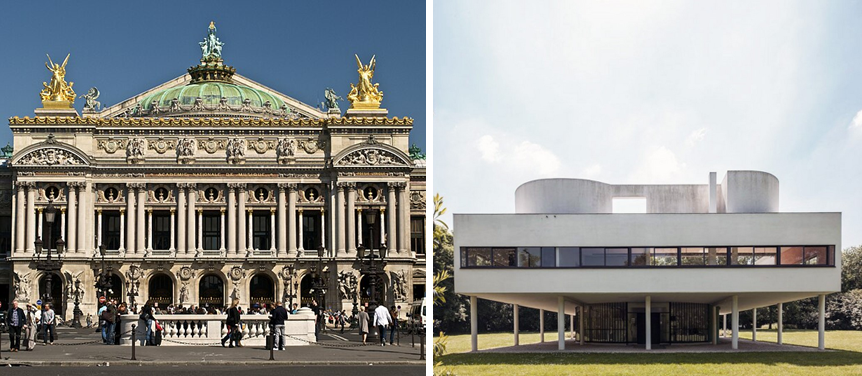
\includegraphics[width= \linewidth]{Images/NeoclassicismVsModernism}
          \caption{Neoclassic building "Paris Opera" 19th AC (left) vs Modernist house "Villa Savoye" 20th AC (right). From Complexity to simplicity. (\textit{Images edited from source:\cite{Stacbond2020}})}
          \label{fig:NeoclassicalvsModernism}
        \end{figure}

This architectural ethos adopted the maxim ``Form follows function'', emphasizing functionalism and characterized by a rejection of traditional ornament in favor of new forms of more subtles intricacies like the “aesthetics of machinery” that showcased architecture  enriched  with  only  the  beauty of its lines and the use of new-age materials such as steel, glass, and concrete\cite{Gage2015}.
Venturi\cite{Venturi1972} further reflects that modern architecture considered as progressive, If not revolutionary, utopian, and puristic;
it  is  dissatisfied  with existing conditions and its architects would prefer to change rather than enhance what is there.

%% add some extra references to the modernist section specially about the urban configuration 

The postmodernism style of the late 60's marks a radical return of ornament in form recognizing that even simplified modern elements serve as ornamentation focusing on the thought of freeing design element from oppresive modern constraints.



The late 20th century embraced imagination and expression through architects like Frank Gehry, Zaha Hadid, and Rem Koolhaas.
Their constructions stood as monumental expressions of ornament, enabled by digital technologies (Figure\ref{fig:Modernismvspostmodernism}).

%%Figure neoclassicim vs modernism
     \begin{figure}[htb]
          \centering
          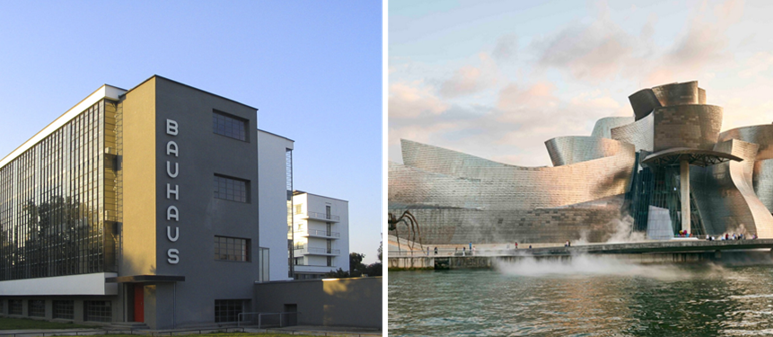
\includegraphics[width= \linewidth]{Images/modernism vs postmodernism}
          \caption{Modernist building "Bauhaus School" 20th AC (left) vs Postmodernist "Guggenheim museum" 1997 (right). From simplicity to Complexity. (\textit{Images edited from source:\cite{Arora2023}})}
          \label{fig:Modernismvspostmodernism}
        \end{figure}

Intricate shapes and structures have materialized, spanning from juxtaposed ornaments to innovative transformative structural ornamentation.
This pursuit of complexity is a global phenomenon, prompting a competitive quest among leading contemporary architectural firms to harness parametric design as a tool to conceive groundbreaking new buildings.\cite{Burlando2019}.

However, due to their complexity, these structures remained exceptional, not integrated into the urban fabric.
Now at the beginning of the 21st century and the advent of the 4th industrial revolution, characterized by a fusion of technologies that is blurring the lines between the physical, digital, and biological spheres\cite{Schwab2016}, forecasts the democratization of digital fabrication which in turn will bring a paradigm shift, offering globally to all cultures the means to express authenticity through complex parametric designs, signaling a contemporary era embracing complexity and ornament.

Amidst this historical exploration, it becomes evident that the architecture of the future is poised to harmonize ornamentation, functionality, and human comfort.
The trajectory points towards a style of complexity—a style that crafts a delicate equilibrium, resonating with the values of our time and the technological possibilities at our fingertips.

In this intricate interplay, architecture emerges as a tangible synthesis of human experience and creative expression, balancing ornament's aesthetic allure, the essential functionality of the built environment, and the crucial comfort of its inhabitants.

\subsection{Cultural Significance of Facades and Ornament}
\label{subsec: FacadeandOrnament}
%%Delve deeper into how facades reflect cultural values, societal norms, and historical contexts. Explore how different societies and civilizations have expressed their identity through architectural ornamentation and symbolism.
We have established a foundation for the notion that contemporary architecture is gravitating towards a renaissance of complexity.
This resurgence is catalyzed by the utilization of technology and sophisticated software analyses, enabling the creation of innovative ornamentation that seamlessly integrates functionality with cultural heritage.
This evolution paves the way for the elaboration of intricate patterns that serve as a powerful medium to express the distinct identity of the local environment, thereby rejuvenating the urban landscape.

Transitioning into the focal point of this research, we delve into the trajectory of architectural complexity within the specific realm of facades.

Facades, a paramount architectural element, have held an enduring significance for centuries due to their role as the initial point of contact with a building, acting as a boundary between the interior and the exterior, working as an interface between the living spaces and the external climate, influencing comfort and energy efficiency\cite{Kamal2020} thereby acting as the primary medium through which the structure interacts with its surroundings (Figure\ref{fig:FacadeBaroqueVsContemporary}).

%% Figure of baroque facade vs contemporary facade
     \begin{figure}[htb]
          \centering
          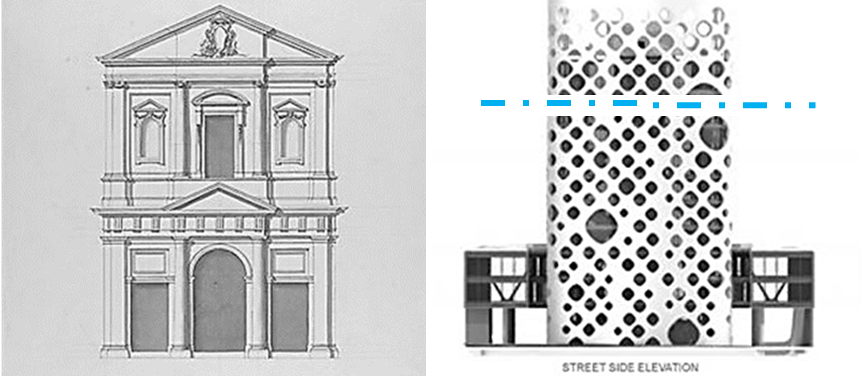
\includegraphics[width= \linewidth]{Images/BaroqueVsContemporaryfacade}
          \caption{Evolution of facade design.
          Baroque Facade 1639 by Bernini (left) vs Contemporary facade, building O-14 by Reiser + Umemoto, 21st Century (right) (\textit{Images edited from source)}}
          \label{fig:FacadeBaroqueVsContemporary}
        \end{figure}

However, much like the broader scope of architecture, the role of ornamentation and facades has also undergone evolution and transformation throughout history.
To elucidate how various societies and civilizations have conveyed their identity through architectural ornamentation and symbolism, we embark on an exploration of the interpretations given to facades by some of the most influential architects and artists of their respective eras.

%%Facade according to vitruvius

Vitruvius, a celebrated Roman architect and military engineer, in 1st century BCE, author of ``De Architecura'', a series of ten books considered as the first treatise in architecture theory\cite{Kruft1994}.
Within this work, Vitruvius advocates for three essential attributes that a building should embody: ``firmitas'' (structural soundness), ``utilitas'' (functionality), and ``venustas'' (beauty or aesthetics)\cite{Ostwald2023}.

Vitruvius places emphasis primarily on Reason, and secondarily on proportions.
It's worth highlighting that the cultural atmosphere in ancient Rome during the late first century B.C favoured the understanding of the world as a well-structured and ordered whole\cite{Lefas2000}.

Facades partake of this reasoning and in accordance to Vitruvius should not only be visually appealing but should also reflect the underlying structural integrity of the building and fulfill its intended purpose effectively(Figure\ref{fig:Vitruvianarchitecture}).
In terms of ornamentation, Vitruvius seeks to approach this subjective realm, dominated by taste, with objectivity.
He rationalizes that a pleasing appearance emerges from the harmony and balance among the components that constitute a composition\cite{Lefas2000}.

%% Figure of vitruvian Architecture
    \begin{figure}[htb]
        \centering
        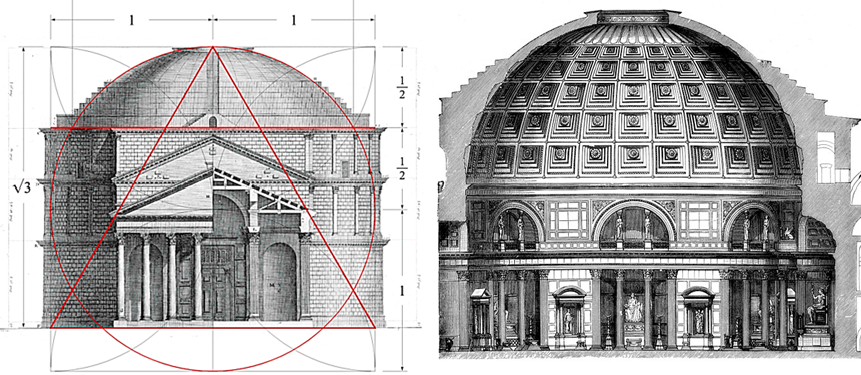
\includegraphics[width= \linewidth]{Images/VitruvianArchitecture}
        \caption{Facade and ornament according to Vitruvius, with emphasis in order symmetry and harmony. Pantheon's facade (left) and cross section(right) symmetry analysis (\textit{Images edited from source)}}
        \label{fig:Vitruvianarchitecture}
    \end{figure}

Additionaly, Vitruvius determines that the deciding factor for those components would follow the principle of ``Decor'',  the  fifth  principle on his system of values that elevates simple  building  practice  into  architecture, defined as the property that  deals  with  the  «appropriate»  articulation and construction of the work on principles respecting religion, nature and social conventions\cite{Lefas2000}.

In essence, according to Vitruvius, facades and their ornamentation stem from a sense of order and rationality.
They are achieved through a harmonious equilibrium of well-considered elements that adhere to established principles, while taking into account both tradition and nature.
This approach aims to achieve beauty while also effectively fulfilling the intended purpose of the facade.

Vitruvius's contributions would have a lasting impact on the field of construction spanning centuries.
However, his work remained largely dormant for a considerable period until its revival during the Renaissance.
This resurgence led to the rekindling of Classical architecture in the years that followed\cite{Wikipedia2023}.

%%facade according to bernini and borromini
Moving beyond the Renaissance era and into the Baroque style, a significant shift in the perception of facades and ornamentation occurs.
Francesco Borromini, a prominent Italian architect of the Baroque period, emerges as a key figure in this context.

In his exploration of facades, Borromini emphasized the dynamic relationship between a building's interior and its facade, as a form of movement of matter beyond the body, precisely because the generation of form is internal to the object itself\cite{Benjamin2006}, therefore the facade should serve as a visual representation of the internal spaces and functions of the building.

Borromini's approach to facades went beyond mere decorative elements.
He saw the facade as an opportunity to express the inner workings and spatial organization of the building.
This concept is reflected in his designs, where facades often featured intricate geometric patterns, curved forms, and sculptural elements that hinted at the internal arrangements of rooms and structures(Figure\ref{fig:BorrominiArchitecture}).

%% Figure of Baroque facade Borromini
     \begin{figure}[htb]
          \centering
          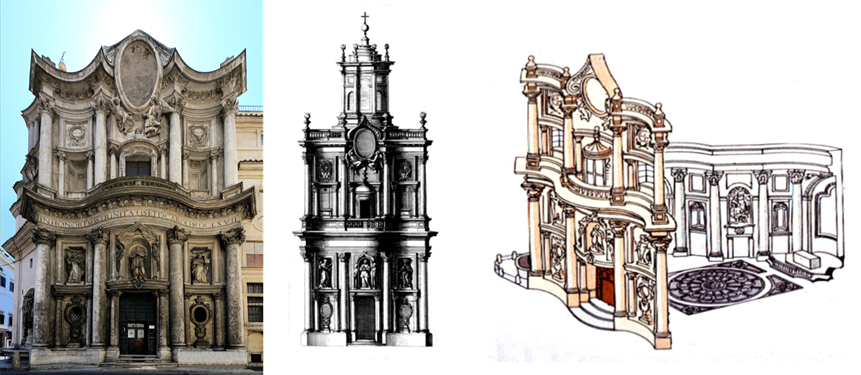
\includegraphics[width= \linewidth]{Images/BaroquefacadeBorromini}
          \caption{Borromini's Interpretation of Facade and Ornament: Elaborate geometric patterns, curved forms, and sculptural elements reflecting internal spatial arrangements. Analysis of San Carlo alle Quattro Fontane Church Facade (left) and Cross Section (right) from its construction in the 1630s, Rome. (\textit{Images edited from source)}}
          \label{fig:BorrominiArchitecture}
        \end{figure}

``Exteriors which expressively display interiorities;
interiors which fold from within and, [\ldots] which appear to invite an exterior reading while presenting an interiorized text''\cite{Biglieri2004}.
In essence, Borromini's perspective on facades went beyond surface aesthetics;
he considered them as integral components of the architectural composition that could convey deeper meanings about the building's design and purpose.

%% context on bypassing neo classic and art deco

By delving into the historical evolution of facades and ornamentation, it's essential to acknowledge certain periods that contributed to our understanding without undergoing radical shifts.
Neo-Classical and Art Deco styles, for instance, added to the discourse around facades and ornament, albeit without fundamentally altering prevailing paradigms .

The Neoclassical style of mid 18th century was a reflection of Facade and Ornament derived from Vitruvian Principles and Palladian Architecture, while the ArtDeco style prevalent in Europe and America during in the 1920s to early 1930s will come to rethink Facade and Ornament through the Prisms of Luxury and Technological Progress.

The goal was to evoke a sense of modernity while also paying homage to the past, resulting in a fusion of historical references and futuristic aspirations (Figure\ref{fig:NeoclassicArtDeco}).

%% Figure of Neo classic style ornament and Art Deco style  facade
     \begin{figure}[htb]
          \centering
          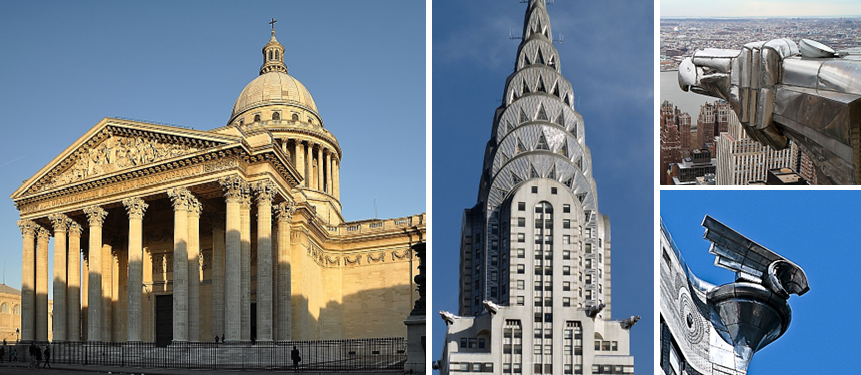
\includegraphics[width= \linewidth]{Images/NeoclassicArtDeco}
          \caption{(Left) Neoclassical Approach in the Mid-18th Century: illustrated by the Paris Pantheon, constructed between 1758 and 1790. (Right) Art Deco Approach in the 1920s to Early 1930s: Exemplified by the Chrysler Building and its Ornamental Details, completed in 1930. (\textit{Images edited from source)}}
          \label{fig:NeoclassicArtDeco}
        \end{figure}

With this broader context established, the analysis will now shift its focus to the Modernist movement's transformative impact on architectural philosophy.

%%facade according to le corbusier

Transitioning from the Baroque style, where facades became expressions of internal dynamics, and acknowledging the enriched insights from the Neoclassical and ArtDeco Style,  the historical evolution of facades and ornamentation takes us into the Modernist style of the 20th century—a pivotal juncture that marked one of the most significant shifts in architectural theory.

 Within this era, a radicalized interpretation of ``Form follows function'' emerged, embodying a profound departure from the conventional understanding of facades and ornamentation, partly due to a prevailing stance against ornamentation, often dismissed on moralistic grounds.

Adolf Loos' 1908 article ``Ornament and Crime'' exemplified this sentiment by advocating functional design and condemning conventional ornamentation as unnecessary\cite{Saglam2014}.

Le Corbusier, one of the most prominent figures of this epoch, and renowned for his influential work ``Towards a New Architecture'' first published in 1923, and considered by some to be the most important architectural work published in the 20th century, epitomized the spirit of the era with his distinct views on facades and ornamentation\cite{Studio2a2023}.

Embracing a minimalist and utilitarian approach, Le Corbusier believed that a facade should mirror a building's internal functions, designed in alignment with its purpose and occupants' needs.

Rooted in a human-centric design philosophy, his mantras ``Constructing the architecture of men'' and ``Men are the ones who truly matter'' underscored his commitment to prioritizing people's well-being in his designs\cite{Virseda2021}.

His manifesto ``The Five Points of a New Architecture'' further solidified his design principles.
The notion of ``Free design of the facade'' attained by separating the exterior of the building from its structural function is presented as the means through which the facade liberates itself from conventional structural\cite{Corbusier1986}.

This allowed for the incorporation of large expanses of windows to provide ample natural light and ventilation, fostering a seamless connection between the interior and exterior realms.

Even during this era when ornamentation was viewed unfavorably, Le Corbusier believes in a form of functional ornamentation, as Venturi\cite{Venturi1972} would later accurately point out, Modern architecture uses expressive ornament and shuns explicit symbolic  ornament.

He would ingeniously devise methods to infuse his creations with a distinct form of ornamentation, albeit one rooted in materials' textures, structural elements, and inventive ways of articulating functionality\cite{Saglam2014} that emerged from the building's design.

For example, he used sunshades, brise-soleil, and other shading devices as a way to address climate and control light without compromising the building's aesthetic integrity.

In essence, Le Corbusier's viewpoint on facades and ornamentation epitomized clarity, rationality, and harmonious integration.
His architecture rejected superfluous adornment, and celebrated both technological advancements and structural innovation while maintaining a genuine focus on the well-being and experiences of the occupants (Figure\ref{fig:Modernistfacade}).

%% Figure of Modernist facade and ornament by Le corbusier
     \begin{figure}[htb]
          \centering
          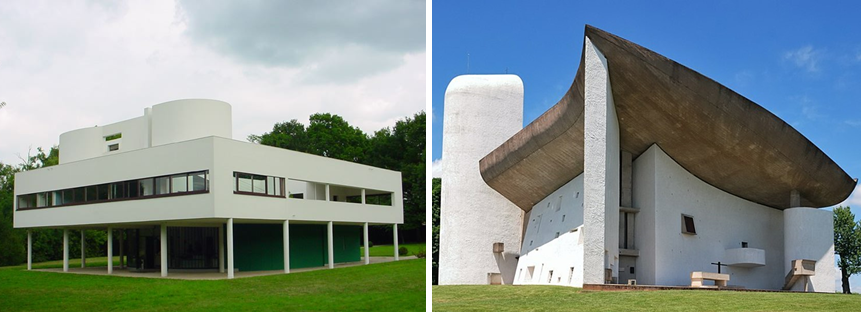
\includegraphics[width= \linewidth]{Images/ModernistFacade}
          \caption{Evolution of Functionalism: Le Corbusier's Journey towards Modernist Facade and Ornamentation. (Left) Villa Savoye, 1928-1931. (Right) Chapelle Notre-Dame-du-Haut de Ronchamp, 1955 (\textit{Images edited from source)}}
          \label{fig:Modernistfacade}
        \end{figure}


%%facade according to Venturi

However, despite the innovative ideals of the Modernist movement,  it became apparent that its utopian vision didn't always materialize as intended.
While the pursuit of functionalism and simplicity was meant to create efficient and logical designs, the outcomes were not always aligned with the intended human experiences.

The Modernist approach often led to the unintentional creation of spaces that felt monotonous and detached from their cultural contexts.
The emphasis on minimalism and the rejection of ornamentation sometimes resulted in environments lacking a sense of identity and character.

The architectural pursuit of universality and timelessness would instead produce sterile, glass-cube structures\cite{Schudel2018} disregarding the importance of cultural heritage and local context, and inadvertently raise the question: Is the reinvention of form, that rejected explicit symbolism and frivolous applique ornament, inspired by the modernist ideals,  yielding a Heroic and original outcome, or is it, instead, a dry expressionism, empty and boring that has distorted the whole building into one big ornament\cite{Venturi1971}.

This scrutiny of the Modernist movement's inability to adequately encompass human experiences and cultural significance, which sparked controversy during the 1960s, brings us to the influential ideas of architect and theorist Robert Venturi.

Venturi's book ``Complexity and Contradiction in Architecture'', published in 1966, marked a turning point in architectural discourse and challenged the prevailing modernist ideals.

Robert Venturi, an iconoclastic architect often hailed as the pioneer of postmodernism\cite{Schudel2018} stood firmly against the oversimplification of architecture, championing the incorporation of contradiction and complexity to yield authentic and vital creations.

The modernist ideals, heavily favoring automobile-centric urban planning, influenced the formation of cities that catered to cars rather than people.
In their thought-provoking book from 1972, "Learning From Las Vegas," Venturi et al.\cite{Venturi1972} put forth a compelling argument, exemplified by the stark contrast seen in places like Las Vegas, they assert that if you were to strip away the dazzling signs, what remains is not a thriving urban environment but a barren desert, illustrating the detachment of architecture relegated to a mere functional necessity camouflaged behind attention-grabbing signs.

Venturi et al.\cite{Venturi1972} will further explain that the oversimplification of architecture, combined with the emergence of sprawling spaces, high speeds, and intricate functions where symbols hold more significance than actual forms, has transformed architecture into symbols occupying space, rather than forming it.

This shift implies that the architectural structure itself carries minimal meaning, with the focus primarily directed towards the signs that communicate with it.

The building stands isolated from the street, often separated by vast parking lots, while the front-facing sign juts out perpendicular to the highway, detached from the building.
At the rear, the structure becomes a utilitarian afterthought, reduced to a budgetary obligation\cite{Venturi1972}.

In this scenario, the absence of signs leaves behind a vacuous atmosphere, characterized by scattered buildings that lack enclosure and cohesion.
The architecture loses its essence, mirroring a cultural void much like a desert devoid of life and enrichment.

The impact of these dynamics is not confined to the past;
instead, they continue to reverberate through the present state of our cities.
Many urban landscapes today still adhere to the principles that emerged from the modernist era.
The prioritization of cars and the resulting sprawling infrastructure persist in shaping cityscapes that often prioritize functionality over human experience.

In response to the challenges posed by the Modernist movement and its unintended consequences, Venturi would reshape the course of architectural discourse.
Notably, he will famously invert the famous dictum of Mies van der Rohe ‘Less is more’ into ‘Less is a bore'\cite{Lutolli2020}, encapsulating his bold departure from the prevailing architectural norms.

In his book ``Complexity and Contradiction in Architecture''\cite{Venturi1977}, Venturi emphasized that architecture should be responsive to the cultural context and the people who inhabit it.

His viewpoint marked a departure from the rigid modernist principles who shunned symbolism of form as an expression or reinforcement of content that dictated that architectural form was to be determined solely by program and structure, with an  occasional  assist from  intuition\cite{Venturi1972}, instead he proposed a reevaluation of the role of ornament and complexity in architectural design (Figure \ref{fig:postmodernfacade}).

%% Figure of Postmodernism facade and ornament
     \begin{figure}[htb]
          \centering
          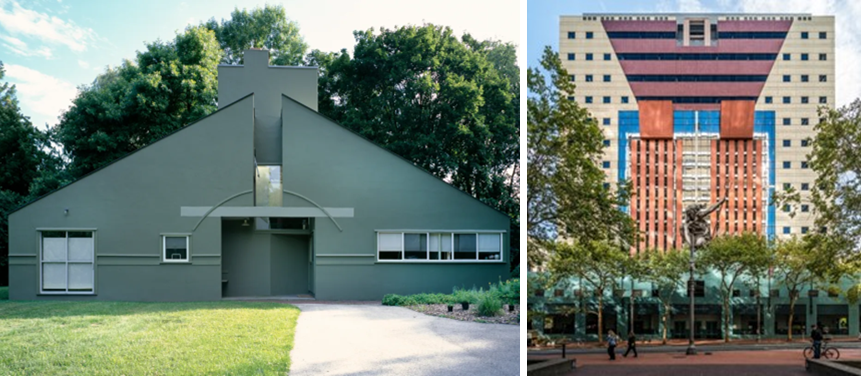
\includegraphics[width= \linewidth]{Images/PostmodernismVenturi}
          \caption{Postmodernism and the advent of complexity and contradiction (Left) Vanna Venturi House, designed by Robert Venturi and Denise Scott Brown in 1964. (Right) Portland Municipal Services Building, designed by Michael Graves, in 1982 (\textit{Images edited from source)}}
          \label{fig:postmodernfacade}
        \end{figure}

Venturi defined facade as ``the principle face of a building, especially the front, which may be architecturally emphasized as a composition or as a plain surface''.
He acknowledged that facades could serve multiple functions beyond just being a simple frontage.
Venturi believed that a facade could communicate various meanings, evoke emotions, and respond to its cultural and contextual surroundings.
He emphasized that facades could be rich in meaning and symbolic expression while simultaneously engaging with the building's interior functions.

Regarding ornament, Venturi's perspective was aligned with his overall rejection of modernist minimalism.
He argued that ornamentation was not inherently negative but should be used judiciously and meaningfully.
Venturi coined the famous phrase ``Less is a bore'', suggesting that architecture doesn't have to be stripped of ornamentation to be considered valid.
He encouraged architects to embrace complexity, contradiction, and the richness of historical references in their designs.

In other words, Robert Venturi's views on facades and ornament emphasized the importance of embracing diversity, historical references, and meaning in architectural design, he wants modern architects to realize only one thing— perfection in the architectural world can and should include imperfection, in all its forms\cite{Lutolli2020}.
=============================
%% reorganize the venturi text and seprate it from the critic of modernism. Add a las vegas analyses pic or something related to the soulless architecture. revision the interpretation of facades and ornament with citations before progressing into the contemporary

%%i need to add a paralel that our cities were generated under the modernist ideals and preference of the car which lead to the reference to Las vegas and how if you remove the signs, there is no place only a desert due to the disengage of architecture now reduce to a cheap necessity hidden behind the sign. Also add a picture of the postmodern style with a reference towards facade and ornament made clear in similar fashion as the conclusions of style written before that ussually start with in essence.

%I want to make a reflection at this point, the modernist movement utopia failed and resulted in the creation of monotonous places desensatized from its culture.
%the functionalism was misinterpreted as plainliness and resulted in dehumanized elements.
%the focus on light and glass facades ignored contextual relationship where the climate unapologetically would turn this glass boxes into ovens pradoxical ignoring the maxim of human centric design.
%architecture would follow a pattern regardless of its roots and connection to its local making them virtually indistinguishable from one another in striking contrast to the richful global diversity of the past.
%the absence of ornament was misinterpreted as the lack of effort reducing architecture to mere construction.

   %%%==========================References


    Venturi wants modern architects to realize only one thing— perfection in the architectural world can and should include imperfection, in all its forms\cite{Lutolli2020}.


    In Complexity and Contradiction in Architecture, Robert Venturi tries to give counter-arguments to the modernist approach. He advocates embracing ‘contradiction and complexity’ to create valid, vital works.\cite{Lutolli2020}

    It is noteworthy that he doesn’t oppose aesthetic simplicity. What he rejects is the ‘oversimplification’ of architecture, indicated when he inverted the famous Mies van der Rohe statement ‘Less is more’ into ‘Less is a bore’.\cite{Lutolli2020}

    Modern architects, who shunned symbolism of form  as  an expression or reinforcement of content: meaning was  to  be  communicated,  not  through  allusion  to  previously  known forms, but through the inherent, physiognomic characteristics of form.
    The creation of architectural form was to be a logical process, free  from images  of past experiences, determined solely by program and structure, with an  occasional  assist,  as  Alan Colquhoun has  suggested, from  intuition.
    But some recent critics  have  questioned  the possible level of content to  be derived  from  abstract forms.
    Others have  demonstrated that the functionalists,  despite  their protestations, derived  a  formal vocabulary of their own, mainly from current art movements and the industrial vernacular;
    and  latter-day  followers  such  as  the  Archigram  group  have turned,  while  similarly  protesting,  to Pop  Art and  the space  industry.\cite{Venturi1972}

    Because the spatial relationships are made by symbols more than by forms, architecture in this landscape becomes symbol in space rather than form in space.
    Architecture defines very little: The big sign and the little building is the rule of Route 66.
    The sign is more important than the architecture.
    This is reflected in the proprietor's budget the sign at the front is a vulgar extravaganza, the building at the back, a modest necessity.
    The architecture is what is cheap.\cite{Venturi1972}

    The little low buildings, gray-brown like the desert, separate and recede from the street that is now the highway, their false fronts disengaged and turned perpendicular to the highway as big, high signs.
    If you take the signs away, there is no place.
    The desert town is intensified communication along the highway.\cite{Venturi1972}

    Ugly and ordinary as symbol and style
    Heroic and Original, or ugly and ordinary

    Robert Venturi, an iconoclastic architect often considered the father of postmodernism who rejected sterile, glass-cube structures in favor of an inclusive, eclectic style that embraced community values and a touch of vulgarity\cite{Schudel2018}

    He turned Mies van der Rohe’s famous dictum about simplicity in design — “Less is more” — upside down, cheekily declaring, “Less is a bore.”\cite{Schudel2018}

    Mr. Venturi’s declaration of architectural values, “Complexity and Contradiction,” was a manifesto that took aim at the prevailing modernist notion that architecture should aspire to a cold, glassy perfection with cold, glassy buildings.
    He argued instead that architecture should reflect changing times and social needs.
    The world of design, he said, had too long been in the grip of the dogma that architects were godlike creators who could impose their vision on the landscape.\cite{Schudel2018}

     Las Vegas wasn’t just a neon-lit den of vulgarity, they concluded.
     It was a prime example of a city built to accommodate the automobile.
     As a result, signs were often more important than the buildings they loomed over.\cite{Schudel2018}

    “In the landscape of the automobile, the architecture becomes insignificant, a pimple on the landscape of parking lots,” Mr. Venturi told the Times in 1971.\cite{Schudel2018}

    He never lost his disdain for what he considered the soulless architecture of his modernist predecessors, who often designed glass-box buildings with walls of windows, “but you would never have a wall with a window in it.”\cite{Schudel2018}

    Instead, Mr. Venturi wrote in “Complexity and Contradiction in Architecture,” he drew inspiration from the “everyday landscape, vulgar and disdained,” which was “valid and vital for our architecture as a whole.”\cite{Schudel2018}

    some architects wanted to move away from minimalist glass and steel and return to the ornamentation of the past. Postmodernists such as Michael Graves, James Stirling, Robert Venturi, and Denise Scott Brown responded to the work of their predecessors with bold buildings that showcased color and references to classical design. [...] Discover five of the most influential buildings of the postmodern movement and see how their eclectic and innovative designs pushed the boundaries of architecture in the 20th century\cite{Stamp2016}.


    %
    According to Krier the mature city achieves balance with nature and with the people that it serves in its scale, size and integration of residential, commercial and civic functions.
    Krier argues that the reconstruction of a city is a moral imperative, a global project that it is at once cultural social economic and ecological. Time of video 1:06:29\cite{Economakis2023}

%%facade according to contemporary Zaha hadid

        ``If architecture is to exist in the 21st century, when attention is focused on the fast-paced worlds of technology, fashion, and entertainment, it must not recede into the background as mere functional equipment''\cite{Gage2015}.

        High-performance building facade systems involve selecting and deploying the right materials, advanced technologies, good detailing, and installation, all of which must be contextually and functionally appropriate.
        It refers to designing buildings and spaces (interior and exterior) using local climatic conditions to improve thermal and visual comfort.\cite{Kamaltech2020}

%%facade according to Bjarke Ingels


\subsection{Digital fabrication and Environmental Sustainability}
\label{subsec:DigitalFabricationAndEnvSustainability}
%8. **Environmental Sustainability:** Investigate how the integration of complex facades and digital fabrication aligns with contemporary sustainability principles. Examine how parametric design and data-driven approaches can enhance energy efficiency, reduce material waste, and contribute to sustainable construction practices.
Digital fabrication technologies, meanwhile, are interacting with the biological world on a daily basis.
Engineers, designers, and architects are combining computational design, additive manufacturing, materials engineering, and synthetic biology to pioneer a symbiosis between microorganisms, our bodies, the products we consume, and even the buildings we inhabit\cite{Schwab2016}.



%%%%
what initially motivates this research is the conscious realization that
Upon delving into the annals of influential architectural styles, a discernible pattern emerges—an oscillation between simplicity and complexity(see Figure\ref{fig:TimelineArchitecture}).
This recurrent cycle in architectural paradigms is not only reflective of the values ingrained in the societies they house, but also closely tied to pivotal technological advancements.
Consider, for instance, the transition from the Romanesque style of the 10th century to the Complex Gothic style 12th style, replaced by the revival of greek and roman ideals during the Renaissence style, followed by the complex opulent ornamentation of the Baroque style in the 16th century replaced by the neoclassical revival of the 18th century, heavily influenced by classical Greek and Palladian architecture\cite{Arora2023}.
This pattern repeats all the way to the 1920s and 30s, the intricate Art Deco will be replaced on the first half of the 20th century witnessed the emergence of Modern Architecture and rationalism emphasizing functionalism and minimalistic architecture




This shift encapsulates the quintessence of architectural evolution—an ever-changing interplay between simplicity and complexity, often steered by the confluence of societal values and technological breakthroughs.


Once again, we find ourselves at a pivotal juncture in history, as the emergence of computer-aided design converges with the industrialization of construction, ushering in a new paradigm in architectural design.
The 20th-century dominance of Rationalism, exemplified by figures like Le Corbusier, underscored an ethos of oversimplification and functionality.
Characterized by straightforward, symmetrical forms and concrete as the favored medium, this era yielded cities estranged from human-centric design.
Swift transportation took precedence, fracturing urban spaces that once defined vibrant societies\cite{Stacbond2020}.
Subsequently, industrial design asserted its dominance as the blueprint for future construction\cite{Economakis2023}, casting architecture in the mold of minimalism and mass-produced uniformity, forsaking the ornate allure and individuality of yesteryears.

\subsection{Object-Oriented Ontology}
\label{subsec:ObjectOrientedOntology}
% add the concept of Object-Oriented. Using these concepts as basis. I want to express that the mr experiment is based on the idea that architecture as a tool should be invisible and confortable while in use. But it should  create emotion when seen as part of the landscape as a form of art to recapture the humand oriented city .
Heideggers tool analysis states that as the tool is a tool it disappears in favor of some purpose he continues to explain that generally we don't notice equipment until it fails, like when An earthquake calls attention to the ground we walk or when a medical problem alerts us of the presence of organs that we have silently depended\cite{Harman2011}.
Harmans, Object-oriented ontology, borrows this concept to formulate its central claim that objects have hidden qualities and realities, and they withdraw from our understanding.\cite{Gage2015}
he idea that we live our lives on a layer of invisible equipment has significant ramifications for architecture, a discipline that produces the equipment on and in which we exist.\cite{Gage2015}


%% End of line numbers
\end{linenumbers}

\pagebreak
%% Start of Bibliography
    \bibliography{main}
    \bibliographystyle{elsarticle-num}

\end{document}